\subsection*{Return to our regular schedule}
We now ask the question, how do we distinguish hyperfinely split $S$ states. The answer is that there is a different total angular momenta for the system in the two different hyperfinely split state.
The measurement scheme is to excite the lower hyperfine S state, to the upper hyperfine D state using a $\pi$ pulse, and continously drive the transition between the upper S state to the lower P state.
If we see a spontaneously emmitted photon, then we will know that we were in the upper state. For practical reasons we must also drive the transition between the lower D and P states.
\begin{figure*}[h]
	\centering
	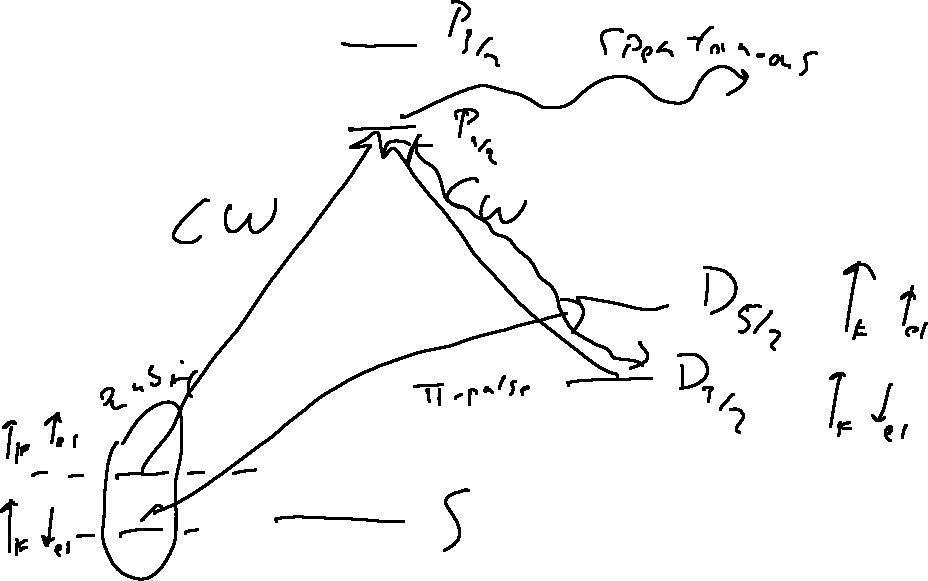
\includegraphics[width=10cm]{12-02-1.png}
	\caption*{The "Shelving" process to distinguish our hyperfinely split state}
\end{figure*}
When performing this measurement clearly we cannot be simultaneously be doing a computation on that qubit.
In order to put ourselves in the lower qubit state, we use optical pumping. 

Optical pumping involves using two different polarizations, which we choose to be left and right circularly polarized light.
Since these two states have angular momentum $S_z = \pm\hbar$. These beams will excite our states ``to the right'' or ``to the left'' diagramatically.
Meanwhile, a photon the is perpendicular to our two beams could be used to lower the state without moving left or right, but this can't drive a transition at $m=0$. We call this $\pi$ polarized.
By driving with a $\pi$ polarized beam, we change states via spontaneous emission of $\sigma_\pm$ polarized light until we arrive at the lower $m=0$ state, after which our state will not transition and we will remain there.
\begin{figure*}[h]
	\centering
	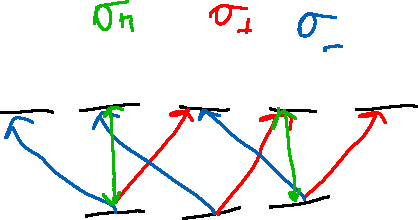
\includegraphics[width=10cm]{12-02-2.png}
	\caption*{The transitions of an atom via differently polarized light fields}
\end{figure*}
\subsection{Superconducting qubits}
Here we will talk about superconductivity, cavity qed, and quantizing electric circuits.

The concept of a quantized circuit raises the question of why circuits don't require quantum mechanics to charactorize normally. This is because the quantum transitions are very low energy, i.e. $kT\gg \hbar\omega_0$. Typical temperatures are $T\approx 15mK$.
In order to have a good quantum system we want $kT \ll \hbar\omega_0$, and $\Gamma\ll\omega_0$

We now seek to quantize the electric circuit, starting from the macroscopic point of view. We begin by looking at the classic LC circuit, which has a resonance at $\omega_0 = \frac{1}{\sqrt{LC}}$.
If we look at typical values pof $L$ and $C$, $L=10nH$, and $C=1pf$, we can see that our frequency is $\omega_0 \approx 1 GHz$. We now take our circuit and quantize it as a harmonic oscillator.
We can add a resistor to our circuit in order to include some dissapation, and this will have a charactoristic time $\tau = RC$. In order to prevent our decay from decohering our quantum system then we want $\tau \gg \omega_0^{-1}$.
Equivalently we can say $R \ll \sqrt{\frac{L}{C}}$. We know that at the temperature we are working at aluminium is superconduction, so we can remove all the resistance of our system by simply using aluminium for all our wires.
Our naive quantization then gives us energy levels $E_n = \frac{\hbar\omega_0}{2}(1+2n)$. Unfortunately this would make an awful qubit, since all energy levels are equally spaced, and therefore we can't distinguish them.

We also want to pick coordinates for our qubit, but this choice isn't immediately clear. Additionally it's unclear why our canonical coordinates would describe our system well at all.
